\section{Neural Ordinary Differential Equations}

In many scientific studies, one often needs to learn how a system behavior changes over time, referred to as the dynamics of the system.
These dynamical systems are modeled using \glspl{ODE} or \glspl{PDE}, similar to the compartmental models introduced in \autoref{sec:literature-review-compartmental-modeling}.
However, its generally challenging to create a model by hand because real-world data are sometimes hard to interpret or are sampled at irregular interval.
Using \glspl{NeuralODE}, the dynamics of the system can be learned through data-driven approaches without having to explicitly specify the \glspl{ODE} or \glspl{PDE}.

Models such as residual networks (see \autoref{fig:residual-network-skip-connection}), \gls{RNN} decoders, or normalizing flows build complex transformations by composing a sequence of modifications to a hidden state \cite{chenNeuralOrdinaryDifferential2019}
\begin{equation*}
    h_{t+1} = h_t + f(h_t, \theta_t)
\end{equation*}
where $t \in \{0 \cdots T\}$ and $h_t \in \mathbb{R}^D$.
These iterative updates can be seen as an Euler discretization of a continuous transformation.
In \gls{NeuralODE}, the continuous dynamics of hidden units are parameterized using an \gls{ODE} specified by an \gls{ANN}
\begin{equation*}
    \frac{dh(t)}{dt} = f(h(t), t, \theta).
\end{equation*}
That is starting from the input layer $h(0)$, the output layer $h(T)$ can be defined as the solution to the \gls{ODE} initial value problem at time step $T$.
There are several benefits when doing this such as memory efficiency, adaptive computation, scalable and invertible normalizing flows, and continuous time-series models.

\begin{figure}
    \centering
    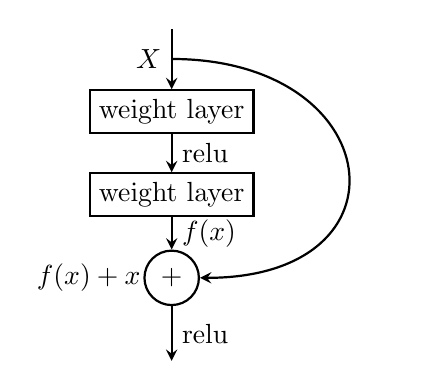
\begin{tikzpicture}[->, >=stealth, node distance = 3em, thick]
        \tikzset{
            block/.style  = {draw, thick, rectangle},
            arith/.style  = {draw, thick, circle},
            input/.style  = {coordinate},
            output/.style = {coordinate}
        }
        \node[input] (IN) {};
        \node[block, below of = IN] (W1) {weight layer};
        \node[block, below of = W1] (W2) {weight layer};
        \node[arith, below of = W2] (ADD) {+};
        \node[output, below of = ADD] (OUT) {+};
        \node[left of = ADD]{$f(x) + x$};

        \draw[->] (IN) to node[left, name=X]{$X$} (W1);
        \draw[->] (X) to [out=0,in=0,looseness=2.5] (ADD);
        \draw[->] (W1) to node[right]{relu} (W2);
        \draw[->] (W2) to node[right]{$f(x)$} (ADD);
        \draw[->] (ADD) to node[right]{relu} (OUT);
    \end{tikzpicture}
    \caption{Example of a skip connection in residual network}
    \label{fig:residual-network-skip-connection}
\end{figure}

For a \gls{NeuralODE} to be trainable with gradient descent, we must have a way to compute the gradients of the loss with respect to the parameters of the \gls{NeuralODE}.
Regular method for taking the loss gradients in \glspl{ANN} (back-propagation) can not be applied for \glspl{NeuralODE} because it incurs high memory cost and introduces additional numerical errors.
Hence, the authors of \cite{chenNeuralOrdinaryDifferential2019} use \textit{adjoint sensitivity analysis} to compute the gradients.
This is done by solving a second, augmented \gls{ODE} backwards in time, and is applicable to all \gls{ODE} solvers.
The approach scales linearly with the problem size, and the numerical error can be controlled explicitly.
\autoref{alg:neural-ode-reverse-mode-diff} shows the overall steps that need to be taken to compute the derivatives.
We consider the loss function $L$, which takes the result of an \gls{ODE} solver
\begin{equation*}
    L(z(t_1)) = L\left(z(t_0) + \int_{t_0}^{t_1}{f(z(t), t, \theta)dt}\right) = L(ODESolve(z(t_0), f, t_0, t_1, \theta)).
\end{equation*}
First, we consider the gradient of the loss with respect to the hidden state $z(t)$, called the adjoint $a(t) = \partial L / \partial z(t)$.
The dynamics of the adjoint is then given by another \gls{ODE}
\begin{equation*}
    \frac{da(t)}{dt} = -a(t)^T\frac{\partial f(z(t), t, \theta)}{\partial z}.
\end{equation*}
The gradient of the loss with respect to the hidden state at the initial time step can be calculated by integrating the adjoint dynamics backwards in time starting from the value $\partial L / \partial z(t_1)$
\begin{equation}
    \frac{dL}{dz(t_0)} = \frac{\partial L}{\partial z(t_1)} + \int_{t_1}^{t_0}{-a(t)^T\frac{\partial f(z(t), t, \theta)}{\partial z}} dt.
    \label{eq:neural-ode-loss-wrt-initial-hidden-state}
\end{equation}
Computing $dL/dz(t_0)$ requires the hidden state $z(t)$ at each evaluated time step which is calculated by integrating the dynamics of our system backwards in time starting from the value $z(t_1)$
\begin{equation}
    z(t) = z(t_1) + \int_{t_1}^{t}{f(z(t), t, \theta)dt}.
    \label{eq:neural-ode-hidden-state-backwards-integral}
\end{equation}
Finally, we can calculate the gradients of the loss function with respect to the parameters $\theta$ using
\begin{equation}
    \frac{dL}{d\theta} = \int_{t_1}^{t_0}{-a(t)^T\frac{\partial f(z(t), t, \theta)}{\partial \theta}} dt.
    \label{eq:neural-ode-loss-wrt-parameters}
\end{equation}
The Jacobian products $a(t)^T\frac{\partial f}{\partial z}$ and $a(t)^T\frac{\partial f}{\partial \theta}$ from \autoref{eq:neural-ode-loss-wrt-initial-hidden-state} and \autoref{eq:neural-ode-loss-wrt-parameters} can be computed efficiently with automatic differentiation.
The integrals in \autoref{eq:neural-ode-loss-wrt-initial-hidden-state}, \autoref{eq:neural-ode-hidden-state-backwards-integral}, and \autoref{eq:neural-ode-loss-wrt-parameters} can be computed in a single call to an \gls{ODE} solver.

\begin{algorithm}
    \caption{Reverse-mode derivative of an ODE initial value problem (taken from \cite{chenNeuralOrdinaryDifferential2019})}
    \label{alg:neural-ode-reverse-mode-diff}
    \begin{algorithmic}
        \Function{ODEDerivative}{$\theta, t_0, t_1, z(t_1), \frac{\partial L}{\partial z(t_1)}$}
            \State $s_0 \gets \left[z(t_1), \frac{\partial L}{\partial z(t_1)}, 0_{|\theta|}\right]$
            \Comment{Define augmented }
            \Function{AugDynamics}{$\left[z(t), a(t), \cdot\right], t, \theta$}
                \State \Return $\left[f(z(t), t, \theta), -a(t)^T\frac{\partial f}{\partial z}, -a(t)^T\frac{\partial f}{\partial \theta}\right]$
            \EndFunction
            \State $\left[z(t_0), \frac{\partial L}{\partial z(t_0)}, \frac{\partial L}{\partial \theta}\right] \gets \Call{ODESolve}{s_0, \textproc{AugDynamics}, t_1, t_0, \theta}$
            \State \Return $\left[\frac{\partial L}{\partial z(t_0)}, \frac{\partial L}{\partial \theta}\right]$
        \EndFunction
    \end{algorithmic}
\end{algorithm}